\documentclass[11pt, oneside]{article} 
\usepackage{geometry}
\geometry{letterpaper} 
\usepackage{graphicx}
	
\usepackage{amssymb}
\usepackage{amsmath}
\usepackage{parskip}
\usepackage{color}
\usepackage{hyperref}

\graphicspath{{/Users/telliott_admin/Dropbox/Tex/png/}}
% \begin{center} 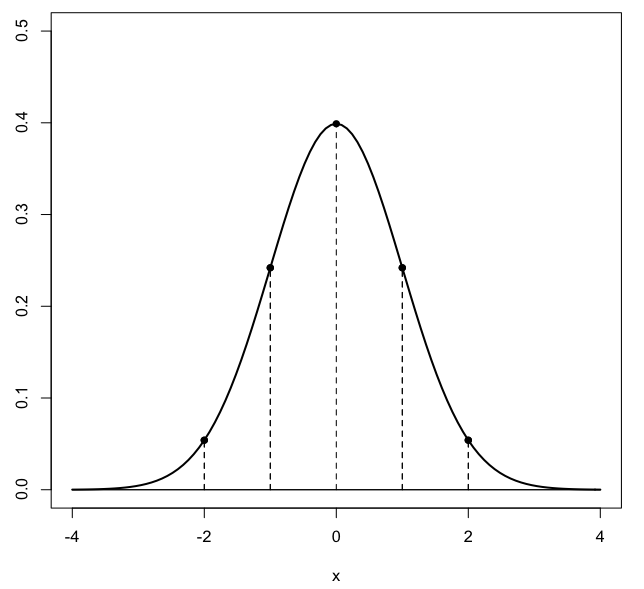
\includegraphics [scale=0.4] {gauss3.png} \end{center}

\title{Partial fractions}
\date{}

\begin{document}
\maketitle
\Large

Strang gives this example:
\[ \int \frac{1}{x-2} + \frac{3}{x+2} - \frac{4}{x} \ dx \]
\[ = \ln |x-2| + 3 \ln |x+2| - 4 \ln |x| \]

That seems straightforward enough.  Which function would produce that sum?
\[ \frac{1}{x-2} + \frac{3}{x+2} - \frac{4}{x}  \]
\[ =\frac{(x+2)(x) + 3(x-2)(x) -4(x-2)(x+2)}{(x-2)(x+2)(x)}  \]
\[ =\frac{x^2 + 2x + 3x^2 - 6x - 4x^2 + 16}{x^3 - 4x}  \]
\[ =\frac{- 4x + 16}{x^3 - 4x}  \]

We call this form $P/Q$, and it's the type of problem we are trying to solve using \emph{partial fractions}.  We start by factoring $Q$ (although sometimes, the factors are given).
\[ Q = x^3 - 4x = x(x^2 -4) \]
\[ = x (x-2) (x+2) \]
Let's try with a different numerator to see how it works.  We write:
\[ \frac{P}{Q} = \frac{3x^2 + 8x -4}{(x-2)(x+2)(x)}  \]
\[ = \frac{A}{x-2} + \frac{B}{x+2} + \frac{C}{x} \]
where $A$,$B$ and $C$ are constants.  

We recognize that we can put these three fractions over $Q$ as the common denominator.

These are the partial fractions that add up to $P/Q$.  We need to find the values of $A$,$B$ and $C$.

Here are two methods (the first one is slower):

Do what we just said.  Put the right-hand side over the common denominator $Q$:
\[ \frac{A}{x-2} + \frac{B}{x+2} + \frac{C}{x} \]
\[ = \frac{A(x+2)(x) + B(x-2)(x) + C(x-2)(x+2)}{(x-2)(x+2)(x)} \]

Now make the numerators match:
\[ 3x^2 + 8x -4 = A(x+2)(x) + B(x-2)(x) + C(x-2)(x+2) \]
\[ = Ax^2 + 2Ax + Bx^2 - 2Bx + Cx^2 - 4C \]

We actually have three equations:
\[ Ax^2 + Bx^2 + Cx^2 = 3x^2 \]
\[ 2Ax - 2Bx = 8x \]
\[ -4C = -4 \]
From the last one $C=1$.  From the first one we have:
\[ A + B + C = 3 \]
\[ A + B = 2 \]
and then
\[ A - B = 4 \]
Add them together to get $2A = 6, so A = 3$ and then $B = -1$.
We obtain finally
\[ \frac{P}{Q} = \frac{3}{x-2} + \frac{-1}{x+2} + \frac{1}{x} \]

\subsection*{second method}

The second approach is called the "cover-up method."  We have:
\[ \frac{3x^2 + 8x -4}{(x-2)(x+2)(x)} = \frac{A}{x-2} + \frac{B}{x+2} + \frac{C}{x} \]
Multiply by $(x-2)$
\[ \frac{3x^2 + 8x - 4}{(x+2)(x)} = (\frac{A}{x-2} + \frac{B}{x+2} + \frac{C}{x}) (x-2) \]
\[ = A +  \frac{B(x-2)}{x+2} + \frac{C(x-2)}{x} \]

Now evaluate at $x=2$
\[ \frac{3(2)^2 + 8(x) - 4}{(2+2)(2)} = \frac{12 + 16 - 4}{8} = 3 = A \]

Notice that we do not need to actually write 
\[ A +  \frac{B(x-2)}{x+2} + \frac{C(x-2)}{x} \]

Nor, in calculating $B$, do we need to write
\[ \frac{A(x+2)}{x-2} + B + \frac{C(x+2)}{x} \]

since we will pick $x$ to zero out those terms, instead, just substitute $x=-2$ into
\[ \frac{3x^2 + 8x - 4}{(x-2)(x)} \]
\[ = \frac{3(-2)^2 + 8(-2) - 4}{(-2-2)(-2)} \]
\[ B = \frac{12 - 16 -4}{8} = \frac{-8}{8} = -1 \]

For $C$ multiply the left-hand side by $x$ and evaluate at $x = 0$ (to make the $A$ and $B$ terms go away):
\[ \frac{3x^2 + 8x -4}{(x-2)(x+2)} = \frac{-4}{-4} = 1 = C \]

\subsection*{same degree}

How about 

\[ \int \frac{3x^2 + 2x + 7}{x^2 + 1} \ dx \]

To use the method, $P$ must be of a lower degree than $Q$, but here they both contain multiples of $x^2$ (degree two).  We separate off the term of $3x^2$ by finding another $3$:
\[ \frac{3x^2 + 2x + 7}{x^2 + 1} = \frac{3x^2 + 3 + 2x + 4}{x^2 + 1} \]
\[ = 3 + \frac{2x + 4}{x^2 + 1} \]

Now we just have to solve:
\[ \int 3 + \frac{2x}{x^2 + 1} + \frac{4}{x^2 + 1} \ dx \]
\[ = 3x + \ln(x^2 + 1) + 4 \tan^{-1} x + C \]

\subsection*{repeated factor}
\[ \frac{2x+3}{(x-1)^2} \]

We have two factors of $x-1$.  Solution:  use $(x-1)^2$ for one of the fractions:
\[ \frac{2x+3}{(x-1)^2} = \frac{A}{x-1} + \frac{B}{(x-1)^2} \]
\[ 2x + 3 = A(x-1) + B \]
set $x=1$, then 
\[ B = 2(1) + 3 = 5 \]
and
\[ 2x + 3 = Ax - A + 5 \]
$A=2$ solves this.

\subsection*{more examples}
These few examples are from wikipedia.  We would like to simplify
\[ \frac{3x+5}{(1-2x)^2} \]
 We suppose that this fraction can be decomposed as follows
\[ \frac{3x+5}{(1-2x)^2} = \frac{A}{(1-2x)^2} + \frac{B}{(1-2x)} \]

We multiply by the term with $B$ to put everything over a common denominator:
\[ \frac{A}{(1-2x)^2} + \frac{B}{(1-2x)} \]
\[ = \frac{A}{(1-2x)^2} + \frac{B(1-2x)}{(1-2x)^2}\]

Getting rid of the denominators altogether
\[ 3x + 5 = A + B(1-2x) \]
Now both the constant terms and the terms in $x$ must be equal:
\[ -2Bx = 3x \]
\[ B = -\frac{3}{2} \]
\[ A + B = 5 \]
\[ A = \frac{13}{2} \]
And so
\[ \frac{3x+5}{(1-2x)^2} = \frac{13/2}{(1-2x)^2} + \frac{-3/2}{(1-2x)} \]
To integrate, we would do this
\[ \int \frac{3x+5}{(1-2x)^2} \ dx = \int \frac{13/2}{(1-2x)^2} \ dx + \int \frac{-3/2}{(1-2x)}  \ dx \]
\[ = \frac{13/4}{(1-2x)} +(3/4) \ln (1-2x) \]

Example 2.
\[ f(x) = \frac{1}{x^2 + 2x - 3} = \frac{1}{(x+3)(x-1)} = \frac{A}{x+3} + \frac{B}{x-1} \]
\[ A(x-1) + B(x+3) = 1 \]
\[ Ax + Bx = 0 \]
\[ A = -B \]
\[ -B + 3B = 1 \]
\[ B = \frac{1}{4} \]
\[ f(x) = \frac{1}{4}( \frac{-1}{x+3} + \frac{1}{x-1} )\]

\end{document}  